\chapter{物质的相变}\label{ch:b1:phase-changes}

水是人人都见过三种状态的物质，
也是世界上大多数发电站的工作流体，
是最早的制冰机的\omterm{def:b1:heat-engines:vapourcycle}{制冷剂}，也是天气的“引擎”。
冰在吸热时熔化，温度却纹丝不动；
水壶在海边于 \qty{100}{\degreeCelsius} 沸腾，在
珠穆朗玛峰上则为 \qty{70}{\degreeCelsius}；密封的极冷瓶装水
轻轻一碰就整体凝固。本章描绘\omterm{def:b1:phase-changes:phase}{纯物质}各相的\omterm{def:b1:work-and-energy:phase}{相图}，
即 $(T, P)$ 图与 $(v, P)$ 图，并给出与之配套的三种工具：
\omterm{thm:b1:phase-changes:lever}{杠杆规则}（各相各占多少）、
\omterm{def:b1:phase-changes:phase}{潜热}（\omterm{def:b1:phase-changes:phase}{相变}所需的能量与熵变）以及
\omterm{thm:b1:phase-changes:clapeyron}{克劳修斯–克拉珀龙关系}（边界线的斜率）。本章最后
指出\omterm{def:b1:work-and-energy:phase}{相图}失效之处：\omterm{def:b1:phase-changes:metastable}{亚稳态}，
天气变化与高压锅的“意外”正源于此。

\section{相与 $(T, P)$ 图}

\begin{definition}[纯物质、相、相变]\label{def:b1:phase-changes:phase}
\index{相}\index{相变}\index{纯物质}\index{潜热}
\emph{纯物质}是由单一化学物种组成的物体。
\emph{相}是物体中物理性质均匀的部分，
如固相、液相、气相（与其液体共存的气体称为
\emph{蒸气}）。\emph{相变}（熔化/凝固、汽化/
液化、升华/凝华）是物质由一种相转变为另一种相的过程；
在压强固定时，它发生于固定温度下，伴随热量交换而温度不变，
交换的热量即为\emph{潜热}。
\end{definition}

\begin{proposition}[平衡相图]\label{prop:b1:phase-changes:PTdiagram}
\index{相图}\index{三相点}\index{临界点}\index{饱和蒸气压}
在 $(T, P)$ 平面上，每一相占据一个区域；两相共存只能发生在
一条曲线上（升华、熔化、汽化），三相共存只能发生在
一点，即\emph{\omterm{prop:b1:phase-changes:PTdiagram}{三相点}}。汽化曲线
$P = P_s(T)$（即\emph{\omterm{prop:b1:phase-changes:PTdiagram}{饱和蒸气压}}）终止于
\emph{\omterm{prop:b1:phase-changes:PTdiagram}{临界点}} $(T_c, P_c)$，越过该点后，液体与气体
不再有区别。对水而言，\omterm{prop:b1:phase-changes:PTdiagram}{三相点}为 \qty{273.16}{K}、\qty{611}{Pa}；
\omterm{prop:b1:phase-changes:PTdiagram}{临界点}为 \qty{647}{K}、\qty{221}{bar}。水的熔化线
向左倾斜（冰的密度小于水）；对几乎所有其他物质，熔化线
向右倾斜。
\end{proposition}
\admitted

\begin{omfigure}
\begin{tikzpicture}[font=\small, x=1cm, y=1cm, >=Stealth]
  \draw[->] (0,0) -- (8.4,0) node[below] {$T$};
  \draw[->] (0,0) -- (0,5.2) node[left] {$P$};
  \coordinate (Tp) at (2.4,1.2);
  \coordinate (C) at (6.8,4.4);
  \draw[omDef, very thick] (0.3,0.08) .. controls (1.4,0.3) .. (Tp);
  \draw[omThm, very thick] (Tp) .. controls (2.2,2.8) .. (1.9,5.0);
  \draw[omProp, very thick] (Tp) .. controls (4.6,1.6) and (6.0,3.0) .. (C);
  \fill (Tp) circle (2pt) node[below right, font=\footnotesize] {三相点 $\mathrm T$};
  \fill (C) circle (2pt) node[above left, font=\footnotesize] {临界点 $\mathrm C$};
  \node at (0.9,3.4) {固相};
  \node at (3.6,4.0) {液相};
  \node at (6.6,0.9) {气相};
  \node[omDef, font=\footnotesize, anchor=north] at (1.3,0.9) {升华};
  \node[omThm, font=\footnotesize, rotate=80] at (1.8,3.3) {熔化};
  \node[omProp, font=\footnotesize, rotate=35] at (5.35,1.9) {汽化};
  \draw[dashed] (0,2.4) node[left, font=\footnotesize] {\qty{1}{atm}} -- (8.0,2.4);
  \fill (2.25,2.4) circle (1.6pt) node[above left, font=\footnotesize, xshift=2pt] {\qty{0}{\degreeCelsius}};
  \fill (5.12,2.42) circle (1.6pt) node[above left, font=\footnotesize] {\qty{100}{\degreeCelsius}};
  \draw[dotted] (C) -- (6.8,0) node[below, font=\footnotesize] {$T_c$};
  \node[font=\footnotesize, align=center] at (7.6,3.3) {超临界 \\ 流体};
\end{tikzpicture}

{\small 水的\omterm{def:b1:work-and-energy:phase}{相图}（未按比例）。在大气压下加热，
沿虚线所示等压线进行：冰在与熔化线相交处熔化，
水在与汽化线相交处沸腾。
水的熔化线向左倾斜：
压强降低其熔点。}
\end{omfigure}

\begin{remark}[沸腾、蒸发与高压锅]\label{rem:b1:phase-changes:boiling}
液体在任何温度下都会从表面\emph{蒸发}，只要其上方
蒸气的分压低于 $P_s(T)$；
当 $P_s(T)$ 达到环境压强时，液体便\emph{沸腾}，
蒸气泡得以在其内部长大。水在 \qty{100}{\degreeCelsius} 沸腾，
是因为 $P_s(\qty{100}{\degreeCelsius}) = \qty{1.013}{bar}$；在
珠穆朗玛峰上，压强为 \qty{0.33}{bar}，水在 \qty{70}{\degreeCelsius} 附近沸腾；
在压强为 \qty{1.8}{bar} 的高压锅中，则在 \qty{117}{\degreeCelsius} 附近沸腾。
沸腾液体的温度由压强锁定——这一事实
用了两个世纪来定义摄氏温标。
\end{remark}

\section{$(v, P)$ 图与杠杆规则}

\begin{proposition}[安德鲁斯等温线]\label{prop:b1:phase-changes:andrews}
\index{安德鲁斯等温线}\index{饱和曲线}
在比体积的克拉珀龙平面 $(v, P)$ 上，等温线
$T < T_c$ 由三部分组成：陡峭的一支（液相，几乎不可压缩），
水平的\emph{平台}，位于 $P = P_s(T)$ 处，液、气两相在此共存，
以及类双曲线的一支（气相）。平台
两端的比体积 $v_l(T)$ 与 $v_v(T)$ 分别是饱和液体与饱和蒸气的比体积；
它们的\omterm{def:b1:point-kinematics:frame}{轨迹}是\emph{\omterm{prop:b1:phase-changes:andrews}{饱和曲线}}（即穹顶），
其顶点即\omterm{prop:b1:phase-changes:PTdiagram}{临界点}，该处温度为 $T_c$ 的等温线
具有水平拐点。高于 $T_c$ 时，平台不复存在。
\end{proposition}
\admitted

\begin{theorem}[杠杆规则]\label{thm:b1:phase-changes:lever}
\index{杠杆规则}\index{干度（蒸气质量分数）}
质量为 $m$、比体积为 $v$ 的物质，在温度 $T$ 下位于平台上时，
分为蒸气质量分数 $x = m_v/m$（即\emph{干度}）的蒸气，
以及质量分数为 $1 - x$ 的液体，满足
\[
v = (1 - x)v_l + x\,v_v , \qquad\text{即}\qquad
x = \frac{v - v_l}{v_v - v_l} = \frac{LM}{LV} ,
\]
这一比值即为状态点 $M$ 在平台上所截两段之比。
对单位质量的任一广延量（$u$、
$h$、$s$），同样的规则成立：$h = (1 - x)h_l + xh_v$。
\end{theorem}

\begin{proof}
体积可加：$V = m_lv_l + m_vv_v$；两边除以 $m$。能量、焓与
熵也都是广延量。
\end{proof}

\begin{omfigure}
\begin{tikzpicture}[font=\small, x=1cm, y=1cm, >=Stealth]
  \draw[->] (0,0) -- (9.4,0) node[below] {$v$};
  \draw[->] (0,0) -- (0,5.4) node[left] {$P$};
  % dome
  \draw[omDef, thick] plot[smooth, tension=0.8] coordinates {(0.7,0.2) (0.8,2.0) (1.3,3.6) (2.6,4.5) (4.0,3.5) (5.2,2.0) (7.0,1.1) (9.0,0.5)};
  \fill (2.6,4.5) circle (2pt) node[above, font=\footnotesize] {$\mathrm C$};
  % isotherm T1 < Tc
  \draw[omProp, thick] (0.62,5.0) .. controls (0.7,3.2) .. (0.8,2.0) -- (5.2,2.0)
        .. controls (6.4,1.6) and (7.6,1.1) .. (9.2,0.85);
  \node[omProp, font=\footnotesize, anchor=west] at (9.0,1.2) {$T_1$};
  % critical isotherm
  \draw[omThm, thick] (1.1,5.3) .. controls (1.8,4.6) and (2.2,4.5) .. (2.6,4.5)
        .. controls (3.6,4.5) and (5.0,3.4) .. (9.2,2.4);
  \node[omThm, font=\footnotesize, anchor=west] at (9.0,2.7) {$T_c$};
  % supercritical isotherm
  \draw[omExo, thick] (1.7,5.4) .. controls (2.6,4.9) and (4.0,4.4) .. (9.2,3.6);
  \node[omExo, font=\footnotesize, anchor=west] at (9.0,3.9) {$T_2 > T_c$};
  % lever
  \fill (0.8,2.0) circle (1.6pt) node[above left, font=\footnotesize] {$L$};
  \fill (5.2,2.0) circle (1.6pt) node[above right, font=\footnotesize] {$V$};
  \fill (2.5,2.0) circle (1.6pt) node[above, font=\footnotesize] {$M$};
  \draw[<->, omDef] (0.8,1.55) -- (2.5,1.55) node[midway, below, font=\footnotesize] {$x\,(v_v - v_l)$};
  \draw[<->, omDef] (2.5,1.55) -- (5.2,1.55) node[midway, below, font=\footnotesize] {$(1 - x)(v_v - v_l)$};
  \draw[dashed] (0.8,2.0) -- (0.8,0) node[below, font=\footnotesize] {$v_l$};
  \draw[dashed] (5.2,2.0) -- (5.2,0) node[below, font=\footnotesize] {$v_v$};
  \draw[dashed] (2.5,2.0) -- (2.5,0) node[below, font=\footnotesize] {$v$};
  \node[font=\footnotesize, rotate=90] at (0.3,3.4) {液体};
  \node[font=\footnotesize] at (3.7,0.6) {液体 + 蒸气};
  \node[font=\footnotesize] at (7.6,0.25) {蒸气};
  \draw[dashed] (0,2.0) node[left, font=\footnotesize] {$P_s(T_1)$} -- (0.8,2.0);
\end{tikzpicture}

{\small 克拉珀龙图上的\omterm{prop:b1:phase-changes:andrews}{安德鲁斯等温线}。穹顶之下的
等温线 $T_1$ 在 $P_s(T_1)$ 处为一平台；其上的状态点 $M$ 为一种
混合态，其蒸气分数 $x$ 为比值 $LM/LV$。临界
等温线在顶点处与穹顶相切，且拐点水平；
高于 $T_c$ 时既无平台，
也无液体与气体之分。}
\end{omfigure}

\begin{example}[水壶与锅炉]\label{ex:b1:phase-changes:lever}
水在 \qty{100}{\degreeCelsius}、\qty{1}{atm} 下：$v_l = \qty{1.04e-3}{m^3/kg}$，
$v_v = \qty{1.67}{m^3/kg}$——比值为 $1600$。一个密闭的 \qty{1.0}{L}
容器中盛有该温度下的 \qty{0.50}{kg} 水，其 $v =
\qty{2.0e-3}{m^3/kg}$，且 $x = (2.0 - 1.04) \times 10^{-3}/1.67 = 5.8 \times 10^{-4}$：
\qty{0.29}{g} 的蒸气占据容器的一半。密闭容器中将蒸气
质量加倍几乎不改变状态点；压强
仅由温度决定。
\end{example}

\section{相变的能量学}

\begin{proposition}[相变的潜热、焓与熵]\label{prop:b1:phase-changes:latent}
\index{相变焓}\index{相变熵}
在共存的温度 $T$ 与压强 $P_s(T)$ 下，由相 1 到相 2 的
单位质量的\omterm{def:b1:phase-changes:phase}{相变}过程是可逆的、
等温、等压，且
\[
L_{12}(T) = h_2 - h_1 , \qquad s_2 - s_1 = \frac{L_{12}}{T} , \qquad
u_2 - u_1 = L_{12} - P_s(v_2 - v_1) .
\]
$L_{12} > 0$，即向较无序的相转变（熔化、
汽化、升华），且 $L_{21} = -L_{12}$。水在 \qty{1}{atm} 下：
$L_f = \qty{334}{kJ/kg}$，在 \qty{0}{\degreeCelsius} 时；$L_v = \qty{2257}{kJ/kg}$，在
\qty{100}{\degreeCelsius} 时。
\end{proposition}

\begin{proof}
定压下所吸收的热量为 $\Delta H$
（见\cref{prop:b1:first-law:qvqp}）；若可逆且等温，则其值为
$T\Delta S$（见\cref{prop:b1:second-law-entropy:identity}）；并有 $U = H - PV$。
\end{proof}

\begin{example}[汽化热的去向]\label{ex:b1:phase-changes:whereheat}
水在 \qty{100}{\degreeCelsius} 下：$P_s(v_v - v_l) = 1.013 \times 10^5 \times
1.67 = \qty{169}{kJ/kg}$，故 $u_v - u_l = 2257 - 169 = \qty{2088}{kJ/kg}$：
\omterm{def:b1:phase-changes:phase}{潜热}的 $93\%$ 用于将分子拉开，$7\%$
用于把大气推回。
汽化熵 $2257/373 = \qty{6.05}{kJ/(kg.K)}$，远大于熔化熵 $334/273 =
\qty{1.22}{kJ/(kg.K)}$：熔化使分子松动，沸腾则使分子脱离束缚。
\end{example}

\begin{method}[含相变的量热法]\label{meth:b1:phase-changes:calorimetry}
在定压绝热容器中，$\sum\Delta H_i = 0$。先猜测
终态（存在哪些相、处于何温度）；
将各物体的 $\Delta H$ 写为显热 $mc\,\Delta T$ 加上\omterm{def:b1:phase-changes:phase}{潜热}
$\pm mL$（依所经历的变化取正负）之和；求解；\emph{检验
猜测}：若某物体终温高于沸点或低于
熔点，或某一相的质量为负，说明猜测有误——此时终态
为\omterm{def:b1:phase-changes:phase}{相变}温度下的混合物，
未知量即为发生\omterm{def:b1:phase-changes:phase}{相变}的质量（见\cref{ex:b1:first-law:ice}）。
\end{method}

\begin{example}[蒸汽烫伤]\label{ex:b1:phase-changes:steam}
\qty{10}{g} 温度为 \qty{100}{\degreeCelsius} 的蒸汽在皮肤上凝结时，
在降温一度之前即放出 $0.010 \times 2257 = \qty{22.6}{kJ}$——
相当于 \qty{10}{g} 沸水降温
\qty{540}{K} 时所放出的热量。这正是蒸汽烫伤远比
同温度的水严重，也解释了为何蒸汽散热器只需很小的质量流量。
\end{example}

\begin{omfigure}
\begin{tikzpicture}[font=\small, x=1cm, y=1cm, >=Stealth]
  \draw[->] (0,0) -- (9.0,0) node[below] {$s$};
  \draw[->] (0,0) -- (0,5.2) node[left] {$T$};
  \draw[omDef, thick] (0.9,0.3) .. controls (1.3,2.6) and (2.6,4.4) .. (4.0,4.6)
        .. controls (5.4,4.4) and (7.0,2.4) .. (8.4,0.3);
  \fill (4.0,4.6) circle (2pt) node[above, font=\footnotesize] {$\mathrm C$};
  % isobar at T1
  \draw[omProp, thick] (0.6,0.35) .. controls (1.1,1.2) .. (1.65,2.6) -- (6.65,2.6)
        .. controls (7.4,3.0) and (8.0,3.6) .. (8.6,4.5);
  \node[omProp, font=\footnotesize, anchor=west] at (8.6,4.6) {等压线 $P_1$};
  \draw[dashed] (1.65,2.6) -- (1.65,0) node[below, font=\footnotesize] {$s_l$};
  \draw[dashed] (6.65,2.6) -- (6.65,0) node[below, font=\footnotesize] {$s_v$};
  \draw[dashed] (0,2.6) node[left, font=\footnotesize] {$T_1$} -- (1.65,2.6);
  \draw[<->, omThm] (1.65,2.9) -- (6.65,2.9) node[midway, above, font=\footnotesize] {$s_v - s_l = L_v/T_1$};
  \fill[omThm!15] (1.65,0) rectangle (6.65,2.6);
  \node[font=\footnotesize, omThm] at (4.15,1.2) {面积 $= L_v$};
  \node[font=\footnotesize] at (1.0,3.9) {液体};
  \node[font=\footnotesize] at (8.3,1.9) {蒸气};
  \node[font=\footnotesize] at (4.15,2.0) {液体 + 蒸气};
\end{tikzpicture}

{\small 同一穹顶在\omterm{def:b1:second-law-entropy:TS}{熵图}中的形状。等压线穿过它时，
表现为长为 $L_v/T$ 的水平线段；线段下方的面积即为
\omterm{def:b1:phase-changes:phase}{潜热}。发电站的循环画在这一平面上，
透平出口处的干度由\omterm{thm:b1:phase-changes:lever}{杠杆
规则}从线段上读出。}
\end{omfigure}

\section{克劳修斯–克拉珀龙关系}

\begin{theorem}[克劳修斯–克拉珀龙]\label{thm:b1:phase-changes:clapeyron}
\index{克劳修斯–克拉珀龙关系}
沿相 1 与相 2 的共存曲线，有
\[
\frac{\dd P_s}{\dd T} = \frac{L_{12}(T)}{T\,(v_2 - v_1)} .
\]
\end{theorem}

\begin{proof}
在穹顶内取单位质量，沿一个无穷小\omterm{def:b1:heat-engines:carnotcycle}{卡诺循环}进行：
完成转变 $1 \to 2$，沿温度 $T + \dd T$ 处的平台，
压强为 $P_s + \dd P_s$（一级近似下吸热 $L_{12}$）；
经一无穷小绝热步降至温度 $T$；再沿
温度 $T$、压强 $P_s$ 处的平台完成逆向转变；再经一绝热步回到初态。该循环可逆，工作于
温度 $T + \dd T$ 与 $T$ 之间的双\omterm{def:b1:heat-engines:machine}{热源}，故其\omterm{def:b1:heat-engines:efficiency}{效率}为 $\dd T/T$
（见\cref{thm:b1:heat-engines:carnot}）；其功，即细矩形的面积，
为 $\dd P_s\,(v_2 - v_1)$。由此可得 $\dd P_s\,(v_2 - v_1)/L_{12} =
\dd T/T$。
\end{proof}

\begin{omfigure}
\begin{tikzpicture}[font=\small, x=1cm, y=1cm, >=Stealth]
  \draw[->] (0,0) -- (8.6,0) node[below] {$v$};
  \draw[->] (0,0) -- (0,4.6) node[left] {$P$};
  \draw[omDef, thick] (0.6,0.2) .. controls (0.75,2.0) and (1.6,3.7) .. (2.6,4.0)
        .. controls (3.6,3.7) and (5.8,1.6) .. (8.2,0.4);
  \fill[omProp!25] (0.92,2.0) -- (4.88,2.0) -- (4.95,2.3) -- (0.9,2.3) -- cycle;
  \draw[omProp, thick] (0.92,2.0) -- (4.88,2.0) node[pos=0.5, below, font=\footnotesize] {$T$, $P_s$};
  \draw[omThm, thick] (0.9,2.3) -- (4.95,2.3) node[pos=0.5, above, font=\footnotesize] {$T + \dd T$, $P_s + \dd P_s$};
  \draw[<->] (6.2,2.0) -- (6.2,2.3) node[midway, right, font=\footnotesize] {$\dd P_s$};
  \draw[dotted] (4.88,2.0) -- (6.3,2.0); \draw[dotted] (4.95,2.3) -- (6.3,2.3);
  \draw[<->] (0.92,1.4) -- (4.88,1.4) node[midway, below, font=\footnotesize] {$v_2 - v_1$};
  \draw[dotted] (0.92,2.0) -- (0.92,1.3); \draw[dotted] (4.88,2.0) -- (4.88,1.3);
  \node[font=\footnotesize, omProp, anchor=west] at (4.0,3.5) {$-W = \dd P_s\,(v_2 - v_1)$, \; $Q_h = L_{12}$};
\end{tikzpicture}

{\small 用于证明\omterm{thm:b1:phase-changes:clapeyron}{克劳修斯–克拉珀龙关系}的无穷小\omterm{def:b1:heat-engines:carnotcycle}{卡诺循环}：
两条相距 $\dd T$ 的平台，由
过短而无法画出的绝热步相连；卡诺定理给出其面积与吸热之比等于
$\dd T/T$。}
\end{omfigure}

\begin{corollary}[液体的饱和蒸气压]\label{cor:b1:phase-changes:vapourpressure}
若蒸气可视为\omterm{def:b1:kinetic-theory:model}{理想气体}且 $v_v \gg v_l$，从而 $v_v - v_l \approx
RT/(MP_s)$，并设 $L_v$ 变化很小，则
\[
\frac{\dd P_s}{P_s} = \frac{ML_v}{R}\,\frac{\dd T}{T^2} , \qquad
\ln\frac{P_s(T)}{P_s(T_0)} = \frac{ML_v}{R}\Bigl(\frac{1}{T_0} - \frac{1}{T}\Bigr) :
\]
蒸气压大致随温度按指数规律增长。对于
接近 \qty{100}{\degreeCelsius} 的水，$ML_v/R = 0.018 \times 2.257 \times 10^6/
8.314 = \qty{4890}{K}$，而 $\dd P_s/\dd T = 2.257 \times 10^6/(373 \times 1.67) =
\qty{3.6}{kPa/K}$：沸腾温度每升高一\omterm{def:b1:kinetic-theory:temperature}{开尔文}，压强需
额外增加 \qty{36}{mbar}。
\end{corollary}

\begin{proof}
将 $v_v - v_l \approx RT/(MP_s)$ 代入定理，并分离
变量，取 $L_v$ 为常数积分。
\end{proof}

\begin{omfigure}
\begin{tikzpicture}
\begin{axis}[omaxis, axis x line=bottom, axis y line=left, width=10.5cm, height=6.2cm,
    xlabel={$T$ (\unit{\degreeCelsius})}, ylabel={$P_s$ (\unit{kPa})},
    xlabel style={at={(axis description cs:0.5,-0.14)}, anchor=north},
    xmin=0, xmax=130, ymin=0, ymax=230, xtick={0,20,...,120}, ytick={50,100,150,200}, samples=120, clip=false]
  \addplot[omDef, thick, domain=0:125] {0.133322*10^(8.07131-1730.63/(233.426+x))};
  \addplot[black, dashed] coordinates {(0,101.3) (100,101.3) (100,0)};
  \addplot[black, dashed] coordinates {(0,33) (71,33) (71,0)};
  \addplot[black, dashed] coordinates {(0,180) (117,180) (117,0)};
  \node[font=\footnotesize, anchor=south west] at (axis cs:2,103) {海平面：\qty{100}{\degreeCelsius}};
  \node[font=\footnotesize, anchor=south west] at (axis cs:2,35) {珠穆朗玛峰（\qty{0.33}{bar}）：\qty{71}{\degreeCelsius}};
  \node[font=\footnotesize, anchor=south west] at (axis cs:2,182) {高压锅（\qty{1.8}{bar}）：\qty{117}{\degreeCelsius}};
\end{axis}
\end{tikzpicture}

{\small 水的\omterm{prop:b1:phase-changes:PTdiagram}{饱和蒸气压}。该曲线近似为
关于 $-1/T$ 的指数函数；沸腾温度即为其
与环境压强相交处的温度。}
\end{omfigure}

\begin{example}[冰刀下的冰]\label{ex:b1:phase-changes:skate}
对于冰–水，$L_f = \qty{334}{kJ/kg}$，且 $v_l - v_s = (1.000 - 1.091)
\times 10^{-3} = \qty{-9.1e-5}{m^3/kg}$：$\dd P/\dd T = 3.34 \times 10^5/(273 \times
(-9.1 \times 10^{-5})) = \qty{-1.3e7}{Pa/K} = \qty{-130}{bar/K}$。一名 \qty{70}{kg}
的滑冰者单脚支撑在长 \qty{30}{cm}、宽 \qty{3}{mm}（$\qty{9}{cm^2}$）的冰刀上，
约产生 \qty{8}{bar} 的压强，使熔点降低 \qty{0.06}{K}。压强熔化并非冰刀滑行的原因（
冰面上本就有一层类液态的薄层，且摩擦生热）；
但负斜率确是真实的，这也正是挂着重物的细丝
能切穿冰块、并在其身后重新冻结的原因。
\end{example}

\section{亚稳态}

\begin{definition}[过冷、过热]\label{def:b1:phase-changes:metastable}
\index{过冷}\index{过热}\index{亚稳态}\index{成核}
一种相可以超出其平衡边界而继续存在：液态水
冷却至 \qty{0}{\degreeCelsius} 以下仍不结冰（\emph{过冷}），
加热至沸点以上仍不沸腾（\emph{过热}），
蒸气压缩至超过 $P_s$ 仍不凝结（过饱和）。
此类\emph{亚稳态}要求不存在\emph{成核}
位点——灰尘、划痕、溶解的气体、冰晶——新相正是在其上
开始形成的；一旦受到扰动，它们便会突然且不可逆地
回到平衡态。
\end{definition}

\begin{example}[过冷的瓶子]\label{ex:b1:phase-changes:supercooled}
干净瓶中静止的水处于 \qty{-8}{\degreeCelsius}，瓶身被轻敲：冰
晶体射穿整瓶水，温度跃升至
\qty{0}{\degreeCelsius}。该过程绝热且迅速，因此显热
$c\,\Delta T$ 使一部分水凝固，所占比例为 $x = c\,\Delta T/L_f = 4.18 \times 8/334 =
0.10$ 的水；产生的熵 $c\ln(273/265) - xL_f/273 =
124 - 122 = \qty{+2}{J/(kg.K)}$，为正值，符合要求。云层中
充满温度低至 \qty{-40}{\degreeCelsius} 的\omterm{def:b1:phase-changes:metastable}{过冷}液滴；飞机
积冰与人工播云都利用了这一性质。
\end{example}

\begin{remark}[助沸石与气泡室]\label{rem:b1:phase-changes:nucleation}
半径为 $r$ 的气泡处于压强为 $P$ 的液体中，其内蒸气压为
$P + 2\sigma/r$（表面张力 $\sigma$，参见本科二年级分册）；该气泡只有在
$P_s(T) > P + 2\sigma/r$ 时才能长大，因此纯净液体处于其沸点时
没有足够小的气泡可以开始长大，于是会\omterm{def:b1:phase-changes:metastable}{过热}数\omterm{def:b1:kinetic-theory:temperature}{开尔文}
后才猛然沸腾，即助沸石所要防止的“暴沸”。助沸石通过
提供充满被困气体的孔穴来防止它。粒子物理中的气泡室
利用的正是同一种不稳定性，只是方向相反：\omterm{def:b1:phase-changes:metastable}{过热}液体
会率先沿电离粒子的径迹沸腾。
\end{remark}

\begin{example}[湿度与结露]\label{ex:b1:phase-changes:dew}
\index{相对湿度}\index{露点}
空气中的水蒸气分压为 $P_v \leq P_s(T)$，
\emph{\omterm{ex:b1:phase-changes:dew}{相对湿度}}为 $P_v/P_s(T)$，\emph{\omterm{ex:b1:phase-changes:dew}{露点}}为
温度，即 $P_s$ 降至 $P_v$ 时的温度。空气温度为 \qty{25}{\degreeCelsius}
（$P_s = \qty{3.17}{kPa}$），\omterm{ex:b1:phase-changes:dew}{相对湿度} $60\%$ 时，$P_v = \qty{1.9}{kPa}$，
$\rho_v = P_vM/(RT) = \qty{14}{g/m^3}$，且任何低于
约 \qty{17}{\degreeCelsius} 的表面上都会结露——如清晨的草叶、冷饮瓶、
浴室镜子。若将同一空气抬升，
则以 \qty{9.8}{K/km} 的速率绝热降温（见\cref{pb:b1:phase-changes:1}），并在
约一千米高处达到\omterm{ex:b1:phase-changes:dew}{露点}：这正是积云平坦底部所在之处。
\end{example}

\section{练习}

\begin{exercise}[$\star$]\label{exo:b1:phase-changes:1}
根据课程中的\omterm{def:b1:work-and-energy:phase}{相图}，判断水在下列条件下所处的相：(a) 在
\qty{20}{\degreeCelsius}、\qty{0.5}{kPa} 压强下；(b) 在 \qty{-5}{\degreeCelsius}
、\qty{1}{bar} 压强下；(c) 在 \qty{400}{\degreeCelsius}、\qty{200}{bar} 压强下；
(d) 在 \qty{0.01}{\degreeCelsius}、\qty{611}{Pa} 压强下。为何水洼在
\qty{20}{\degreeCelsius} 时仍会干涸，而水却“在 100 ℃ 沸腾”？
\end{exercise}

\begin{exercise}[$\star$]\label{exo:b1:phase-changes:2}
将 \qty{100}{g}、\qty{100}{\degreeCelsius} 的水蒸气通入
\qty{1.0}{kg}、\qty{20}{\degreeCelsius} 的水中，容器绝热。
求终温（$L_v = \qty{2257}{kJ/kg}$，$c = \qty{4.18}{kJ/(kg.K)}$）。
并与加入 \qty{100}{g}、\qty{100}{\degreeCelsius} 的水的情形作比较。
\end{exercise}

\begin{exercise}[$\star$]\label{exo:b1:phase-changes:3}
一个容积为 \qty{2.0}{L} 的刚性容器内装 \qty{1.0}{kg} 水，温度为
\qty{150}{\degreeCelsius}，处于液–蒸气平衡（$P_s =
\qty{4.76}{bar}$，$v_l = \qty{1.09e-3}{m^3/kg}$，$v_v = \qty{0.393}{m^3/kg}$）。
求干度、蒸气质量及液体所占的体积。
\end{exercise}

\begin{exercise}[$\star$]\label{exo:b1:phase-changes:4}
求水在 \qty{100}{\degreeCelsius} 时的汽化熵，分别以每千克
及每\omterm{def:b1:kinetic-theory:scales}{摩尔}的值表示；并求 \qty{0}{\degreeCelsius} 时每\omterm{def:b1:kinetic-theory:scales}{摩尔}的熔化熵。许多
普通液体的每\omterm{def:b1:kinetic-theory:scales}{摩尔}汽化熵接近
\qty{88}{J/(mol.K)}（特鲁顿规则）：水是否属于普通液体？
\end{exercise}

\begin{exercise}[$\star\star$]\label{exo:b1:phase-changes:5}
求珠穆朗玛峰峰顶处水的沸点，其中 $P =
\qty{0.33}{bar}$，利用\cref{cor:b1:phase-changes:vapourpressure}，取
$ML_v/R = \qty{4890}{K}$；并求在 \qty{2000}{m}（$P = \qty{0.80}{bar}$）处的沸点。
煮 \qty{3}{min} 的鸡蛋会怎样？
\end{exercise}

\begin{exercise}[$\star\star$]\label{exo:b1:phase-changes:6}
求高压锅内的温度，其阀门在绝对压强 \qty{1.8}{bar} 时开启；
若阀门设在 \qty{2.5}{bar}，则同样求出。
\qty{1.8}{bar} 下水蒸气的 $v_v = \qty{0.98}{m^3/kg}$：
容积为 \qty{6}{L} 的高压锅，在 \qty{4}{L} 水上方含有多少克水蒸气？
\end{exercise}

\begin{exercise}[$\star\star$]\label{exo:b1:phase-changes:7}
求水在 \qty{0}{\degreeCelsius} 时熔化曲线的斜率（$L_f =
\qty{334}{kJ/kg}$，$v_s = \qty{1.091e-3}{m^3/kg}$，$v_l = \qty{1.000e-3}{m^3/kg}$）。
冰在 \qty{-1}{\degreeCelsius} 时于何压强下熔化？位于
厚 \qty{3}{km} 冰盖底部的冰（$\rho = \qty{917}{kg/m^3}$）：求
此处的熔化温度，并说明其对冰川流动的一个影响。
\end{exercise}

\begin{exercise}[$\star\star$]\label{exo:b1:phase-changes:8}
一千克的水在 \qty{100}{\degreeCelsius}、
\qty{1}{atm} 压强下全部汽化（$v_v = \qty{1.673}{m^3/kg}$，$v_l = \qty{1.04e-3}{m^3/kg}$）。
求水所接受的功、所吸收的热量，以及水的 $\Delta U$、$\Delta H$、$\Delta S$，
并求热量取自温度为
\qty{1500}{K} 的火焰时所产生的熵。
\end{exercise}

\begin{exercise}[$\star\star$]\label{exo:b1:phase-changes:9}
饱和压强：\qty{1.23}{kPa}（\qty{10}{\degreeCelsius}）、\qty{1.70}{kPa}
（\qty{15}{\degreeCelsius}）、\qty{2.34}{kPa}（\qty{20}{\degreeCelsius}）、\qty{3.17}{kPa}
（\qty{25}{\degreeCelsius}）、\qty{4.24}{kPa}（\qty{30}{\degreeCelsius}）。房间
温度为 \qty{22}{\degreeCelsius}，\omterm{ex:b1:phase-changes:dew}{相对湿度}为 $70\%$：求蒸气压、
\omterm{ex:b1:phase-changes:dew}{露点}（用插值法求）以及 \qty{50}{m^3} 空气中水蒸气的质量；
一块温度为 \qty{12}{\degreeCelsius} 的窗玻璃会否起雾？
若将房间加热至 \qty{25}{\degreeCelsius}（不加水），求新的
\omterm{ex:b1:phase-changes:dew}{相对湿度}。
\end{exercise}

\begin{exercise}[$\star\star\star$]\label{exo:b1:phase-changes:10}
\emph{\omterm{prop:b1:phase-changes:PTdiagram}{三相点}。}(a) 由 $h$ 的状态函数性质，证明在\omterm{prop:b1:phase-changes:PTdiagram}{三相点}处
$L_s = L_f + L_v$（升华 = 熔化 +
汽化）。(b) 利用克劳修斯–克拉珀龙方程，证明升华曲线
在\omterm{prop:b1:phase-changes:PTdiagram}{三相点}处比汽化曲线更陡
（$v_s$、$v_l$ 相对 $v_v$ 可忽略）。(c) 对于水，$L_f = \qty{334}{kJ/kg}$，
$L_v = \qty{2500}{kJ/kg}$，$T = \qty{273.16}{K}$，$P = \qty{611}{Pa}$，蒸气视为
\omterm{def:b1:kinetic-theory:model}{理想气体}，求两条斜率（以 \unit{Pa/K} 为单位）。(d) 为何雪
在干燥寒冷的日子里会消失，却从未融化？
\end{exercise}

\begin{exercise}[$\star\star\star$]\label{exo:b1:phase-changes:11}
\emph{\omterm{def:b1:phase-changes:metastable}{过热}的水。}半径为 $r$ 的气泡位于压强为
$P_0$ 的水中，气泡内蒸气压强为 $P_0 + 2\sigma/r$，其中 $\sigma = \qty{0.059}{N/m}$
（在本阶段不加证明地承认）。（a）求在水中能够长大的气泡的最小半径，已知水温为
\qty{105}{\degreeCelsius}、压强为 \qty{1.013}{bar}，取
$\dd P_s/\dd T = \qty{3.6}{kPa/K}$。（b）在 \qty{101}{\degreeCelsius} 下求同一问题。
（c）一杯水在微波炉中\omterm{def:b1:phase-changes:metastable}{过热}至 \qty{105}{\degreeCelsius}，
被勺子扰动，求瞬间变为水蒸气的水所占的比例，
以及每升水产生的水蒸气体积——并评论
其危险性。（d）沸石为何能防止这种现象？
\end{exercise}

\begin{exercise}[$\star\star\star$]\label{exo:b1:phase-changes:12}
\emph{\omterm{def:b1:heat-engines:vapourcycle}{制冷剂}的循环。}一台\omterm{def:b1:heat-engines:machine}{热泵}以 R-134a 为工质，
沿 \cref{def:b1:heat-engines:vapourcycle} 所示的循环运行：蒸发温度为
\qty{-10}{\degreeCelsius}（\qty{2.0}{bar}；$h_l = \qty{187}{kJ/kg}$，$h_v =
\qty{392}{kJ/kg}$），冷凝温度为 \qty{40}{\degreeCelsius}（\qty{10.2}{bar}；
$h_l = \qty{256}{kJ/kg}$，$h_v = \qty{419}{kJ/kg}$）。工质离开
冷凝器时为饱和液体，离开蒸发器时为饱和蒸气；
压缩机使其焓为 $h = \qty{430}{kJ/kg}$。假定在
节流阀中 $h$ 守恒，压缩机每千克所做的功为
$\Delta h$（稳流平衡，见本科二年级分册）；在换热器中，
等压，$q = \Delta h$（\cref{prop:b1:first-law:qvqp}）。（a）蒸发器入口处的
干度。（b）蒸发器中每千克工质吸收的热量，
冷凝器中放出的热量，压缩功；验证热力学第一定律。
（c）求 $e_p$ 与 $e_f$；与两饱和温度之间的
卡诺值进行比较。（d）供热功率为 \qty{6}{kW} 时的质量流量。
\end{exercise}

\begin{omfigure}
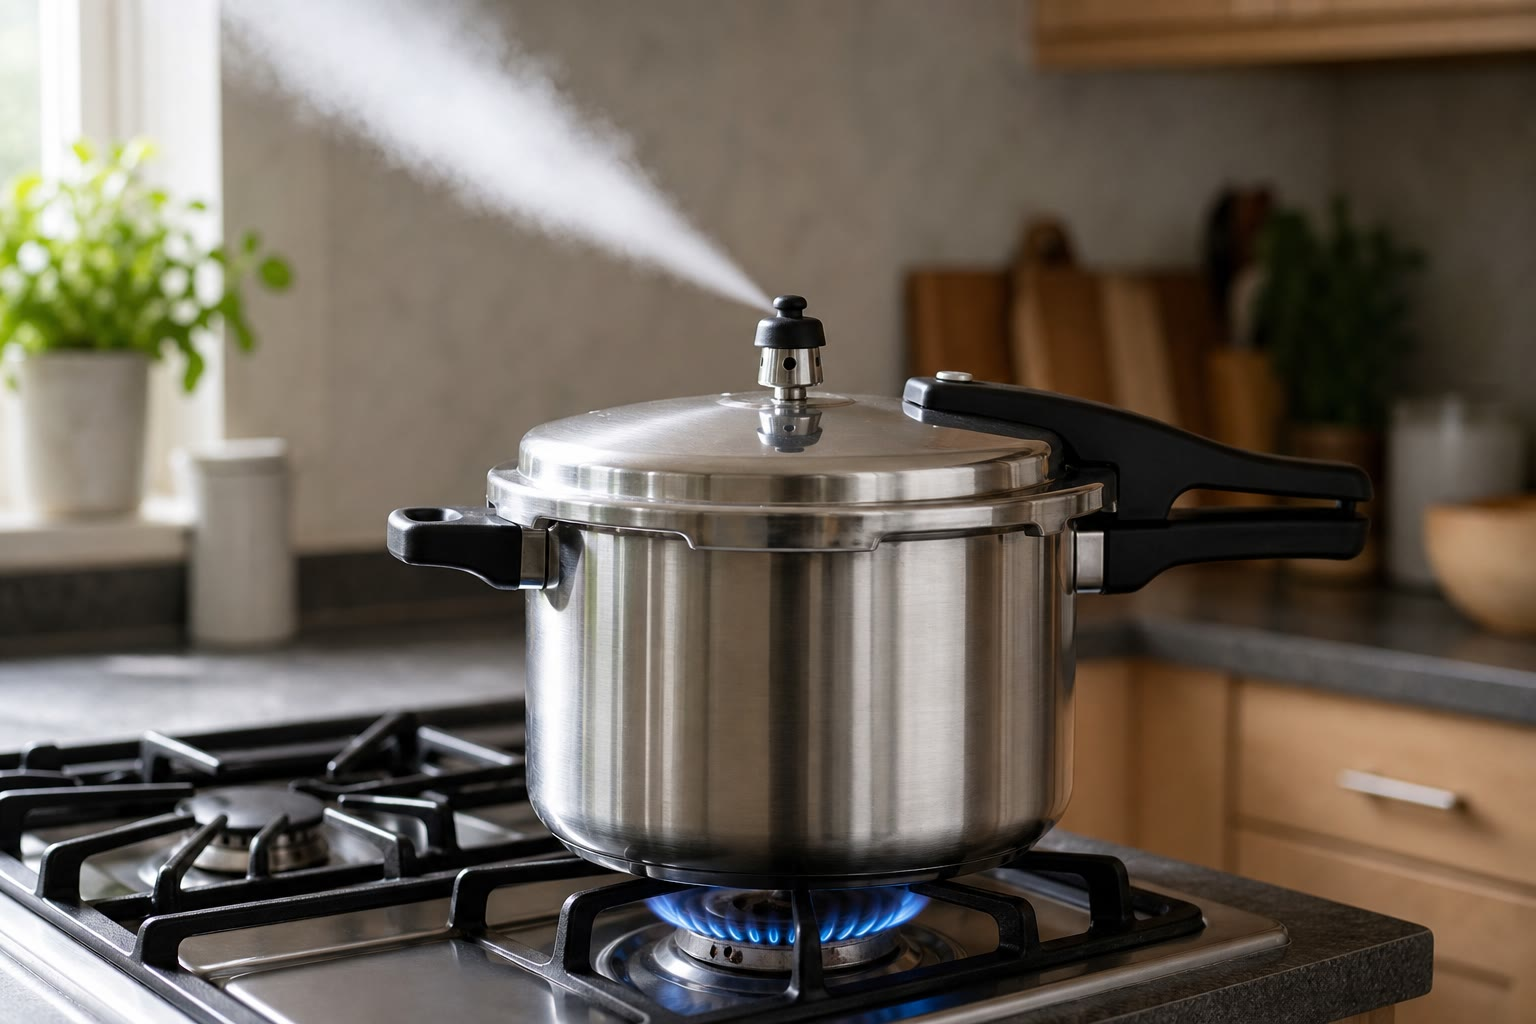
\includegraphics[width=0.58\linewidth]{images/book3/ai/b3-25-pressure-cooker-steam.jpg}

{\small 高压锅：在 \qty{1.8}{bar} 下水于 \qty{117}{\degreeCelsius} 沸腾，压强由限压阀决定。}
\end{omfigure}

\section{问题：四个场景中的水}

\begin{problem}[{周末问题——高压锅、云、
密闭容器与过冷瓶子：同一种物质，其相图的
四种应用}]
\label{pb:b1:phase-changes:1}
水的数据：$L_v = \qty{2257}{kJ/kg}$（\qty{100}{\degreeCelsius}），
在 \qty{117}{\degreeCelsius} 时约为 \qty{2.2}{MJ/kg}，在 \qty{20}{\degreeCelsius} 附近为 \qty{2.45}{MJ/kg}；
$L_f = \qty{334}{kJ/kg}$；$c = \qty{4.18}{kJ/(kg.K)}$
（液态）；$M = \qty{18}{g/mol}$；$ML_v/R = \qty{4890}{K}$，在
\qty{100}{\degreeCelsius} 附近。\omterm{prop:b1:phase-changes:PTdiagram}{饱和蒸气压}：\qty{0.61}{kPa}
（\qty{0}{\degreeCelsius}），\qty{1.23}{kPa}（\qty{10}{\degreeCelsius}），\qty{1.70}{kPa}（\qty{15}{\degreeCelsius}），
\qty{2.34}{kPa}（\qty{20}{\degreeCelsius}），\qty{3.17}{kPa}（\qty{25}{\degreeCelsius}），\qty{4.24}{kPa}
（\qty{30}{\degreeCelsius}），\qty{101.3}{kPa}（\qty{100}{\degreeCelsius}）。
饱和比体积：$v_l = \qty{1.0e-3}{m^3/kg}$（冷水），
\qty{1.9e-3}{m^3/kg}（\qty{360}{\degreeCelsius}）；$v_v = \qty{0.0217}{m^3/kg}$
（\qty{300}{\degreeCelsius}），$0.0108$（\qty{340}{\degreeCelsius}），$0.0088$
（\qty{350}{\degreeCelsius}）；\omterm{prop:b1:phase-changes:PTdiagram}{临界点}为 \qty{374}{\degreeCelsius}，
\qty{221}{bar}，$v_c = \qty{3.1e-3}{m^3/kg}$。空气：$M = \qty{29}{g/mol}$，$c_p =
\qty{1.0}{kJ/(kg.K)}$，$\gamma = 1.4$；$g = \qty{9.8}{m/s^2}$；$R =
\qty{8.314}{J/(mol.K)}$。

\medskip
\noindent\textbf{第一部分——高压锅。}
\begin{enumerate}
  \item 为何海平面处敞口锅中的水无论火焰多强，
        都不能被加热至高于 \qty{100}{\degreeCelsius}？
  \item 从\omterm{thm:b1:phase-changes:clapeyron}{克劳修斯–克拉珀龙关系}出发，推导
        $\ln[P_s(T)/P_s(T_0)] = (ML_v/R)(1/T_0 - 1/T)$，
        并说明所用的近似。
  \item 求阀门开启压强为 \qty{1.8}{bar} 的锅内温度，
        此处为绝对压强。
  \item 限压阀为压在面积为 \qty{20}{mm^2} 的出气口上的重物；
        大气压强为 \qty{1.0}{bar}，求重物的质量。
  \item 用 \qty{2.0}{kW} 的电热盘，将 \qty{2.0}{L} 水由 \qty{20}{\degreeCelsius}
        加热至工作温度（忽略锅的热容）；
        求所需的热量与时间。
  \item 到达后保持电热盘功率为 \qty{2.0}{kW}，求每分钟
        从阀门排出的蒸气质量。厨师应如何操作？
  \item 烹饪反应的速率每升高 \qty{10}{K} 约增大一倍，
        高压锅可将海平面处需 \qty{30}{min} 的菜谱缩短几倍？
        在珠穆朗玛峰上（水在 \qty{70}{\degreeCelsius} 沸腾），
        该菜谱需要多长时间？
\end{enumerate}

\medskip
\noindent\textbf{第二部分——云。}
\begin{enumerate}[resume]
  \item 定义\omterm{ex:b1:phase-changes:dew}{相对湿度}。求 \qty{25}{\degreeCelsius}、$60\%$ 空气中的
        水蒸气分压，以及每立方米中水蒸气的质量
        （视为\omterm{def:b1:kinetic-theory:model}{理想气体}）。
  \item 求该空气的\omterm{ex:b1:phase-changes:dew}{露点}（用表格插值）。解释清晨草叶上的露水
        以及冷瓶外壁上水滴的成因。
  \item 一团干燥空气上升时与外界无热量交换。由可逆绝热定律及
        静力学关系
        $\dd P/\dd z = -\rho g$，证明 $\dd T/\dd z = -g/c_p$，并
        计算其数值。
  \item 随压强降低，上升气团自身的\omterm{ex:b1:phase-changes:dew}{露点}约
        以每千米 \qty{2}{K/km} 的速率下降。求
        第~8~题中的气团达到饱和的高度，即云底。
  \item 在云底之上，凝结的水蒸气将其\omterm{def:b1:phase-changes:phase}{潜热}释放给气团。
        每千克空气中凝结 \qty{1}{g} 水，能使该空气升温多少？
        这对继续上升的气团的冷却速率有何影响，
        以及这一效应
        为何对雷暴至关重要？
  \item 一朵体积为 \qty{1}{km^3} 的积云，每立方米含 \qty{1}{g} 液态水：
        求水的质量，以及其凝结释放的能量，
        分别以焦耳和 \unit{GW h} 表示。
  \item 浴室镜子温度为 \qty{18}{\degreeCelsius}，空气温度为
        \qty{25}{\degreeCelsius}、\omterm{ex:b1:phase-changes:dew}{相对湿度} $80\%$：镜面会起雾吗？
        \omterm{ex:b1:phase-changes:dew}{相对湿度}为多少时会停止起雾？
\end{enumerate}

\medskip
\noindent\textbf{第三部分——密封容器。}
一个容积为 \qty{1.0}{L} 的刚性钢容器中装有质量为 $m$ 的水，
不含空气，密封后缓慢加热。
\begin{enumerate}[resume]
  \item 当 $m = \qty{0.50}{kg}$、温度为 \qty{20}{\degreeCelsius} 时：内部压强，
        比体积，水蒸气的质量（$v_v$ 按\omterm{def:b1:kinetic-theory:model}{理想气体}计算），
        以及液体所占容积的比例。
  \item 加热后液面是上升还是下降？大约在何温度下液体充满整个容器，
        此后压强怎样变化？
        （$v_l$ 取 \qty{360}{\degreeCelsius} 时的值。）
  \item 当 $m = \qty{0.10}{kg}$ 时：加热时液面上升还是下降？
        大约在何温度下最后一滴水蒸发？
        （用 $v_v$ 表计算。）
  \item 当 $m = \qty{0.31}{kg}$ 时：描述温度趋近 \qty{374}{\degreeCelsius} 时
        观察者在弯月面处所见的现象。
  \item 在 $(v, P)$ 图中画出三条加热路径的草图，并标出饱和穹顶，
        说明每条路径
        经过\omterm{prop:b1:phase-changes:PTdiagram}{临界点}的哪一侧。
  \item 同一 \qty{1.0}{L} 容器装入 \qty{0.50}{kg} 水，
        并\emph{连同}其原有的、\qty{20}{\degreeCelsius}、\qty{1.0}{bar} 下的空气一起密封，
        加热至 \qty{100}{\degreeCelsius}：求内部总压强（道尔顿定律），
        以及作用在面积为 \qty{100}{cm^2} 盖板上的力。
\end{enumerate}

\medskip
\noindent\textbf{第四部分——\omterm{def:b1:phase-changes:metastable}{过冷}的瓶子。}
\begin{enumerate}[resume]
  \item 一瓶洁净、静置的水已冷却至 \qty{-8}{\degreeCelsius}
        而未凝固。这种状态叫什么？为何可能出现，
        轻敲瓶子时会发生什么？
        为何温度随后恰好稳定在 \qty{0}{\degreeCelsius}？
  \item 求凝固的水所占的比例（过程很快，故
        可视为绝热）。
  \item 求每千克水产生的熵，并检验其符号。
  \item 反过来看：一杯水在微波炉中加热至 \qty{105}{\degreeCelsius} 而未沸腾，
        随后被扰动。求瞬间变为水蒸气的水所占比例，
        每升水所产生的蒸气体积
        （$v_v = \qty{1.67}{m^3/kg}$），以及杯子为何会喷溅。
  \item 损失的功：一升\omterm{def:b1:phase-changes:metastable}{过冷}水本可与 \qty{0}{\degreeCelsius} 的外界一起
        构成一台可逆\omterm{def:b1:heat-engines:machine}{热机}；取
        $T_0 = \qty{273}{K}$，因轻敲而凝固所浪费的功
        为 $T_0S_{\text{产生}}$。求每升的数值，并
        与将瓶子举高一米的功相比较。结论：\omterm{def:b1:phase-changes:metastable}{亚稳态}
        储存了什么？
\end{enumerate}
\end{problem}
